\documentclass[../Kamil_Kowalewski_Main.tex]{subfiles}

\begin{document} {

    Do eksperymentów został wykorzystany zbiór przedstawiony w~sekcji
    \ref{chapter4:srodowisko_eksperymentalne:zbiory_danych:3}

    \begin{table}[H]
        \scriptsize
        \centering
        \begin{tabularx}{\linewidth}{|L|c|c|c|c|}
            \hline
            % @formatter:off
            Nazwa & Eksperyment \#1 & Eksperyment \#2 & Eksperyment \#3 & Eksperyment \#4 \\ \hline
            Nazwa algorytmu & KMeansEvaluator & FuzzyCMeansEvaluator & BenchmarkEvaluator & BenchmarkEvaluator \\ \hline
            Czas wykonania (s) & 5.875 & 2.11 & 2.0 & 1.922 \\ \hline
            Liczba ofert określona jako wiarygodne & 8 & 8 & 10 & 8 \\ \hline
            Liczba ofert określona jako niewiarogodne & 13 & 13 & 11 & 13 \\ \hline
            % @formatter:on
        \end{tabularx}
        \caption
        [Statystyki dla zbioru danych \#3]
        {Statystyki dla zbioru danych \#3}
    \end{table}

    \begin{figure}[H]
        \centering
        \begin{minipage}[b]{0.49\textwidth}
            \centering
            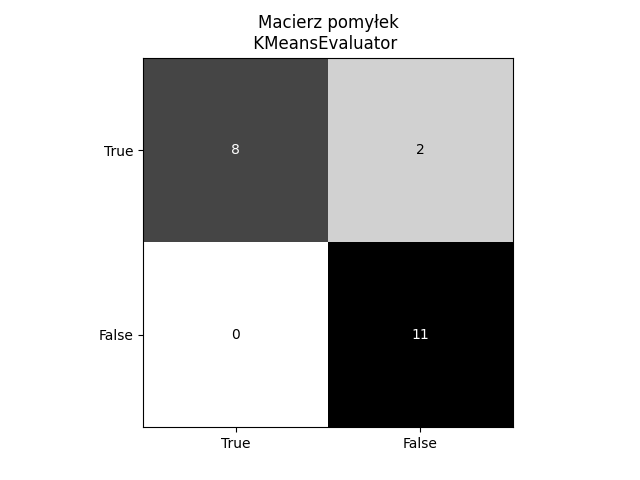
\includegraphics
            [width=\textwidth,keepaspectratio]
            {img/chapter5/dataset3/AppleiPhone11128gb_KMeansEvaluator.png}
            \caption
            [Macierz pomyłek dla zbioru danych \#3, eksperyment \#1]
            {Macierz pomyłek dla zbioru danych \#3, eksperyment \#1}
            \label{fig:chapter5:eksperymenty:zbior:3:eksperyment:1:macierz}
        \end{minipage}
        \hfill
        \begin{minipage}[b]{0.49\textwidth}
            \centering
            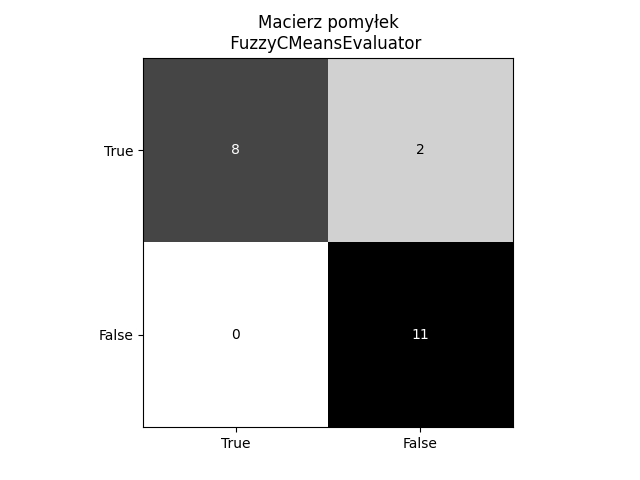
\includegraphics
            [width=\textwidth,keepaspectratio]
            {img/chapter5/dataset3/AppleiPhone11128gb_FuzzyCMeansEvaluator.png}
            \caption
            [Macierz pomyłek dla zbioru danych \#3, eksperyment \#2]
            {Macierz pomyłek dla zbioru danych \#3, eksperyment \#2}
            \label{fig:chapter5:eksperymenty:zbior:3:eksperyment:2:macierz}
        \end{minipage}
    \end{figure}

    \begin{figure}[H]
        \centering
        \begin{minipage}[b]{0.49\textwidth}
            \centering
            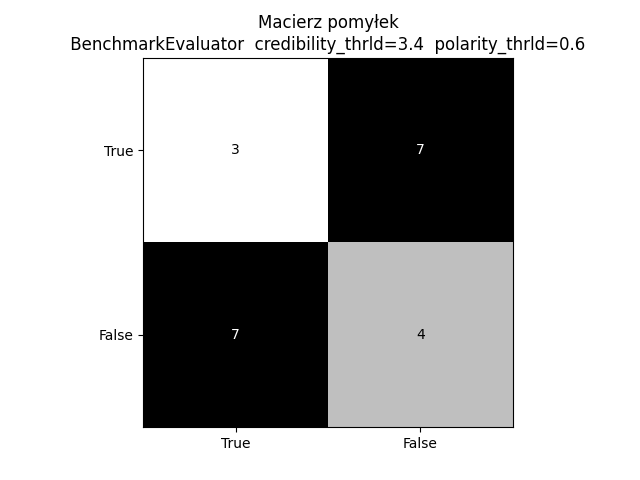
\includegraphics
            [width=\textwidth,keepaspectratio]
            {img/chapter5/dataset3/AppleiPhone11128gb_BenchmarkEvaluator.png}
            \caption
            [Macierz pomyłek dla zbioru danych \#3, eksperyment \#3]
            {Macierz pomyłek dla zbioru danych \#3, eksperyment \#3}
            \label{fig:chapter5:eksperymenty:zbior:3:eksperyment:3:macierz}
        \end{minipage}
        \hfill
        \begin{minipage}[b]{0.49\textwidth}
            \centering
            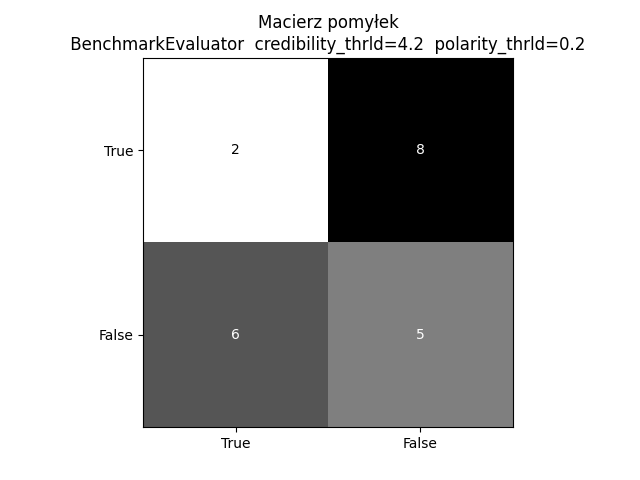
\includegraphics
            [width=\textwidth,keepaspectratio]
            {img/chapter5/dataset3/AppleiPhone11128gb_BenchmarkEvaluator-1.png}
            \caption
            [Macierz pomyłek dla zbioru danych \#3, eksperyment \#4]
            {Macierz pomyłek dla zbioru danych \#3, eksperyment \#4}
            \label{fig:chapter5:eksperymenty:zbior:3:eksperyment:4:macierz}
        \end{minipage}
    \end{figure}

    \subsection{Podsumowanie uzyskanych wyników}
    \label{chapter5:eksperymenty:zbior:1:podsumowanie} {
        Dla autorskiej metody uzyskane wyniki są analogiczne jak dla zbioru danych \#2
        jedynie liczba błędów pierwszego rodzaju zmniejszyła się o~jeden i~wynosi dwa.
        Czasy wykonania analogiczne do zbioru danych \#1.

        Metoda z~literatury popełniła bardzo dużo błędów i~wyniki nie są akceptowalne.
        Dla eksperymentu \#3 było to 7~błędów pierwszego rodzaju i~7~błędów drugiego
        rodzaju natomiast dla eksperymentu \#4 odpowiednio 8~i~6~błędów. Czasy
        wykonania bardzo zbliżone. Można stwierdzić, że skuteczność autorskiej metody
        jest akceptowalna.
    }

}
\end{document}
